\appendix

\section{Appendix / supplemental material}

\subsection{Other single samples visualizations}

% ORIGINAL FIGURE WITH LINE PLOT DESCRIPTION

% \begin{figure}[htb]
%     \centering
%     \begin{subfigure}[b]{.35\textwidth}
%         \centering
%         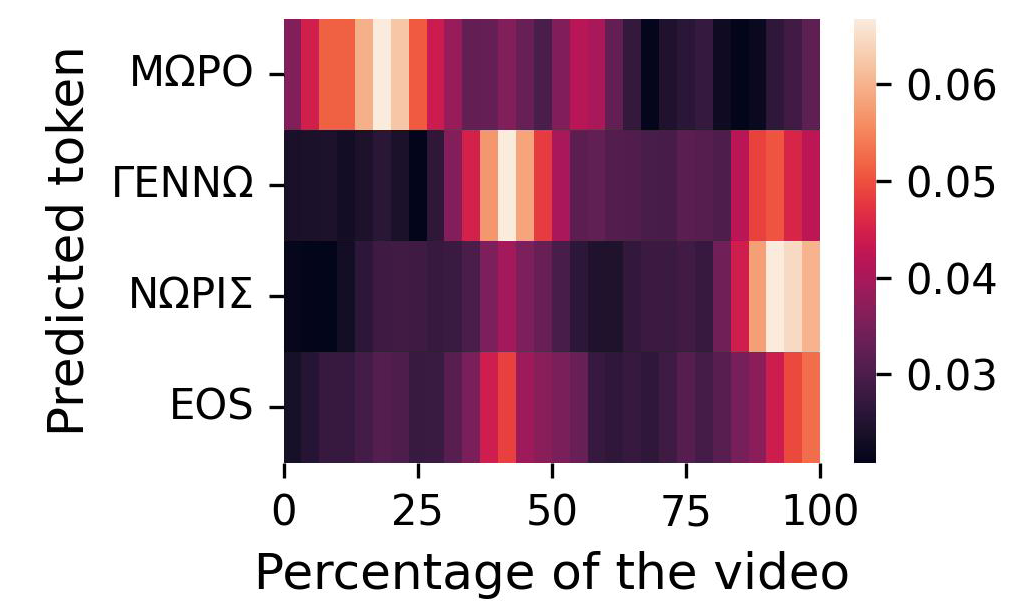
\includegraphics[width=\linewidth]{assets/examples/decoder_ca_heatmap_fh_layer0_idx509.png}
%         \caption{}%Heatmap illustrating the cross-attention distribution across frames for each predicted token in the output sequence. Brighter regions indicate higher attention weights, highlighting which video frames are most significant for each gloss.}
%         \label{subfig:decoder_ca_ex_1_heatmap}
%     \end{subfigure}\hfill
%     \begin{subfigure}[b]{.65\textwidth}
%         \centering
%         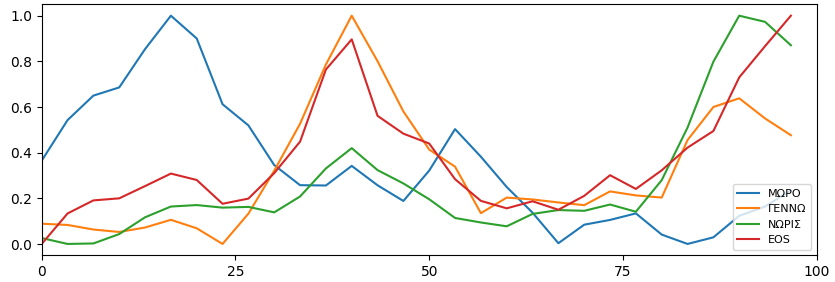
\includegraphics[width=\linewidth]{assets/examples/decoder_ca_lineplot_fh_layer0_idx509.png}
%         \caption{}%Line plot representing the normalized attention weights over the video sequence. The peaks indicate the frames that the model focused on most for each token prediction.}
%         \label{subfig:decoder_ca_ex_1_lineplot}
%     \end{subfigure}
%     %\caption{Visualization of cross-attention mechanisms in the decoder. The heatmap (a) shows the distribution of attention across frames for each predicted gloss, the bar chart (b) displays the normalized attention values from (a) across the pose sequence, and the line plot. The x-axis for (a) and (b) corresponds to the percentage of the video frames.}
%     \caption{Visualization of cross-attention mechanisms in the decoder. (a) Heatmap illustrating the cross-attention distribution across frames for each predicted token in the output sequence. Brighter regions indicate higher attention weights, highlighting which video frames are most significant for each gloss. (b) Line plot representing the normalized attention weights over the video sequence. The peaks indicate the frames that the model focused on most for each token prediction. The x-axis for (a) and (b) corresponds to the percentage of the video frames.}
%     \label{fig:decoder_ca_ex_1}
% \end{figure}

\begin{figure}[htb]
    \centering
    \begin{subfigure}[b]{.375\textwidth}
        \centering
        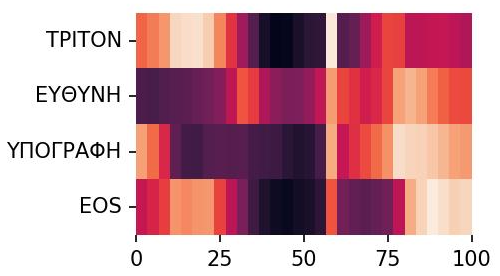
\includegraphics[width=\linewidth]{assets/examples/appendix/171h.png}
        \caption{}
        \label{subfig:subfig1}
    \end{subfigure}\hfill
    \begin{subfigure}[b]{.625\textwidth}
        \centering
        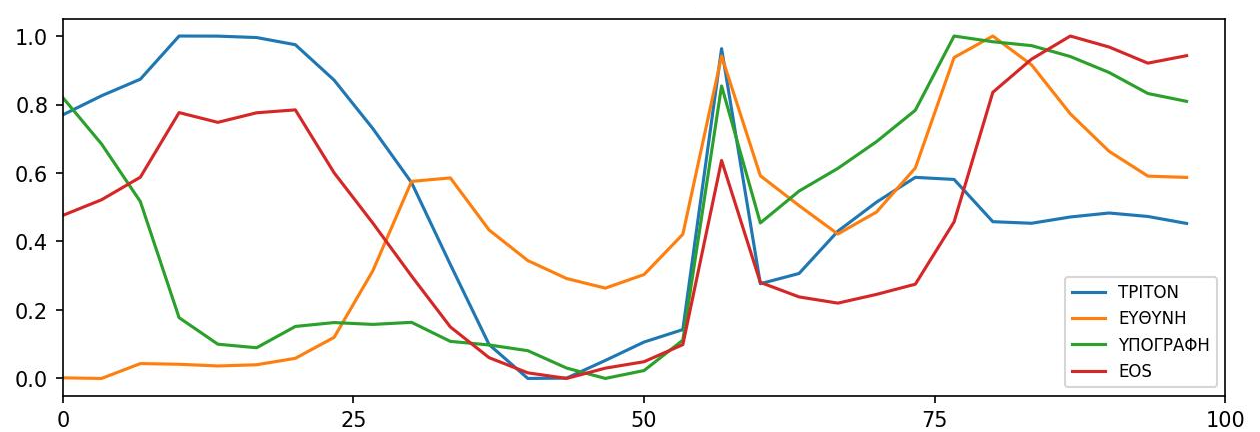
\includegraphics[width=\linewidth]{assets/examples/appendix/171lp.png}
        \caption{}
        \label{subfig:subfig2}
    \end{subfigure}
    \begin{subfigure}[b]{.375\textwidth}
        \centering
        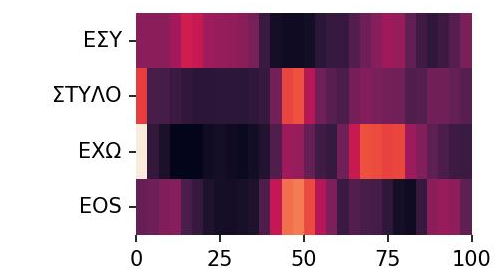
\includegraphics[width=\linewidth]{assets/examples/appendix/447h.png}
        \caption{}
        \label{subfig:subfig3}
    \end{subfigure}\hfill
    \begin{subfigure}[b]{.625\textwidth}
        \centering
        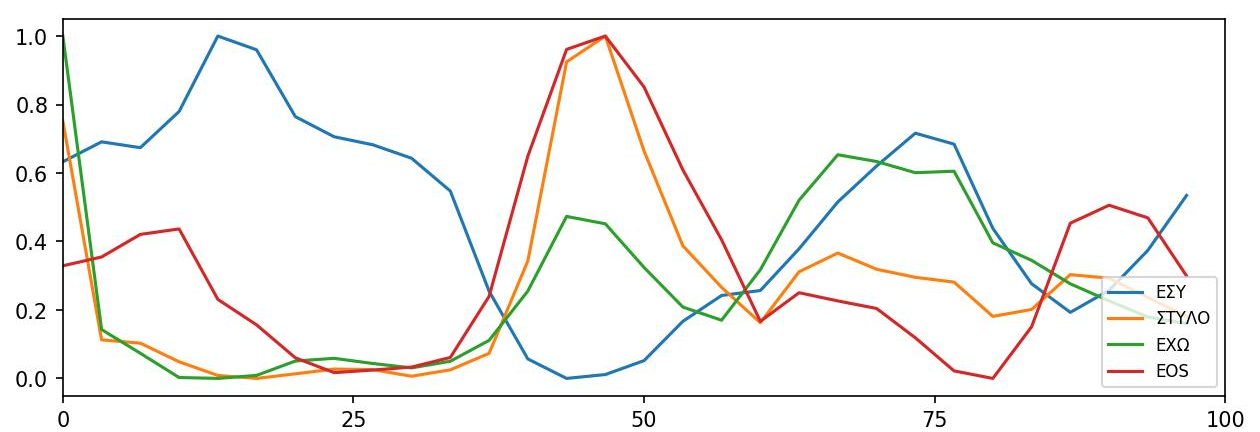
\includegraphics[width=\linewidth]{assets/examples/appendix/447lp.png}
        \caption{}
        \label{subfig:subfig4}
    \end{subfigure}
    \begin{subfigure}[b]{.375\textwidth}
        \centering
        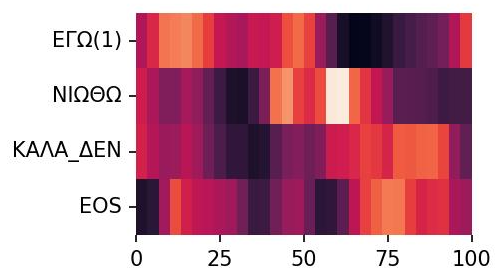
\includegraphics[width=\linewidth]{assets/examples/appendix/618h.png}
        \caption{}
        \label{subfig:subfig5}
    \end{subfigure}\hfill
    \begin{subfigure}[b]{.625\textwidth}
        \centering
        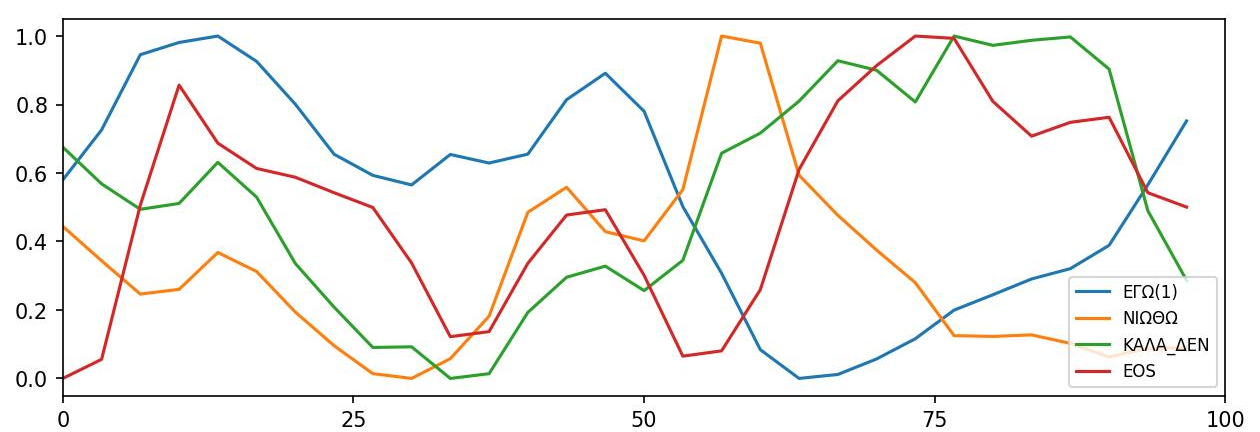
\includegraphics[width=\linewidth]{assets/examples/appendix/618lp.png}
        \caption{}
        \label{subfig:subfig6}
    \end{subfigure}
    \begin{subfigure}[b]{.375\textwidth}
        \centering
        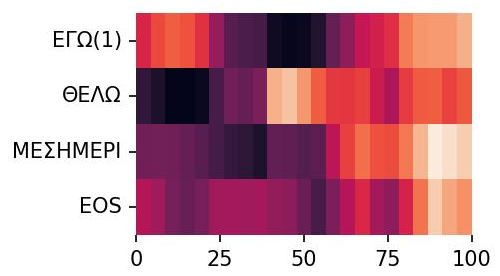
\includegraphics[width=\linewidth]{assets/examples/appendix/819h.png}
        \caption{}
        \label{subfig:subfig7}
    \end{subfigure}\hfill
    \begin{subfigure}[b]{.625\textwidth}
        \centering
        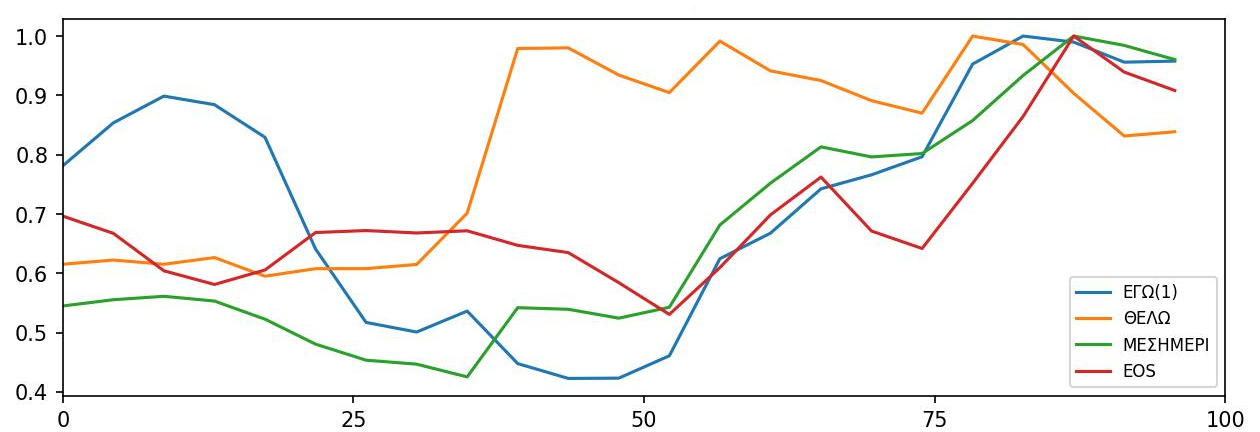
\includegraphics[width=\linewidth]{assets/examples/appendix/819lp.png}
        \caption{}
        \label{subfig:subfig8}
    \end{subfigure}
    \begin{subfigure}[b]{.44\textwidth}
        \centering
        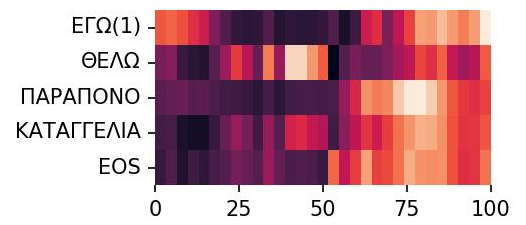
\includegraphics[width=\linewidth]{assets/examples/appendix/31h.png}
        \caption{}
        \label{subfig:subfig9}
    \end{subfigure}\hfill
    \begin{subfigure}[b]{.56\textwidth}
        \centering
        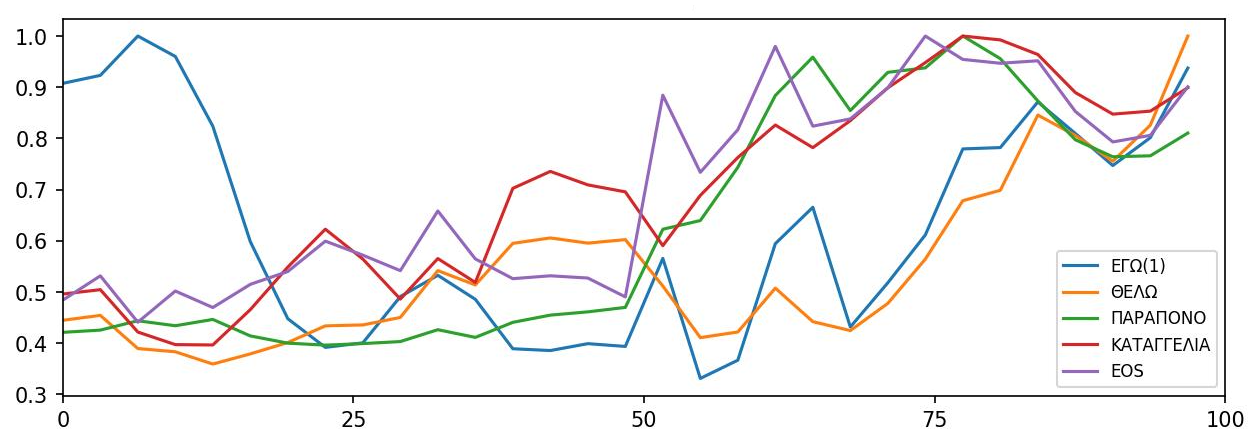
\includegraphics[width=\linewidth]{assets/examples/appendix/31lp.png}
        \caption{}
        \label{subfig:subfig10}
    \end{subfigure}
    \caption{Examples of visualization of cross-attention mechanisms in the decoder. On the left, a heatmap illustrating the cross-attention distribution across frames for each predicted token in the output sequence. On the right, a line plot representing the normalized attention weights over the video sequence. The peaks indicate the frames that the model focused on most for each token prediction.}
    \label{fig:decoder_ca_ex_1}
\end{figure}

\newpage

\subsection{Sign-to-text model results}

\begin{figure}[htb]
    \centering
    \begin{subfigure}[b]{\textwidth}
        \centering
        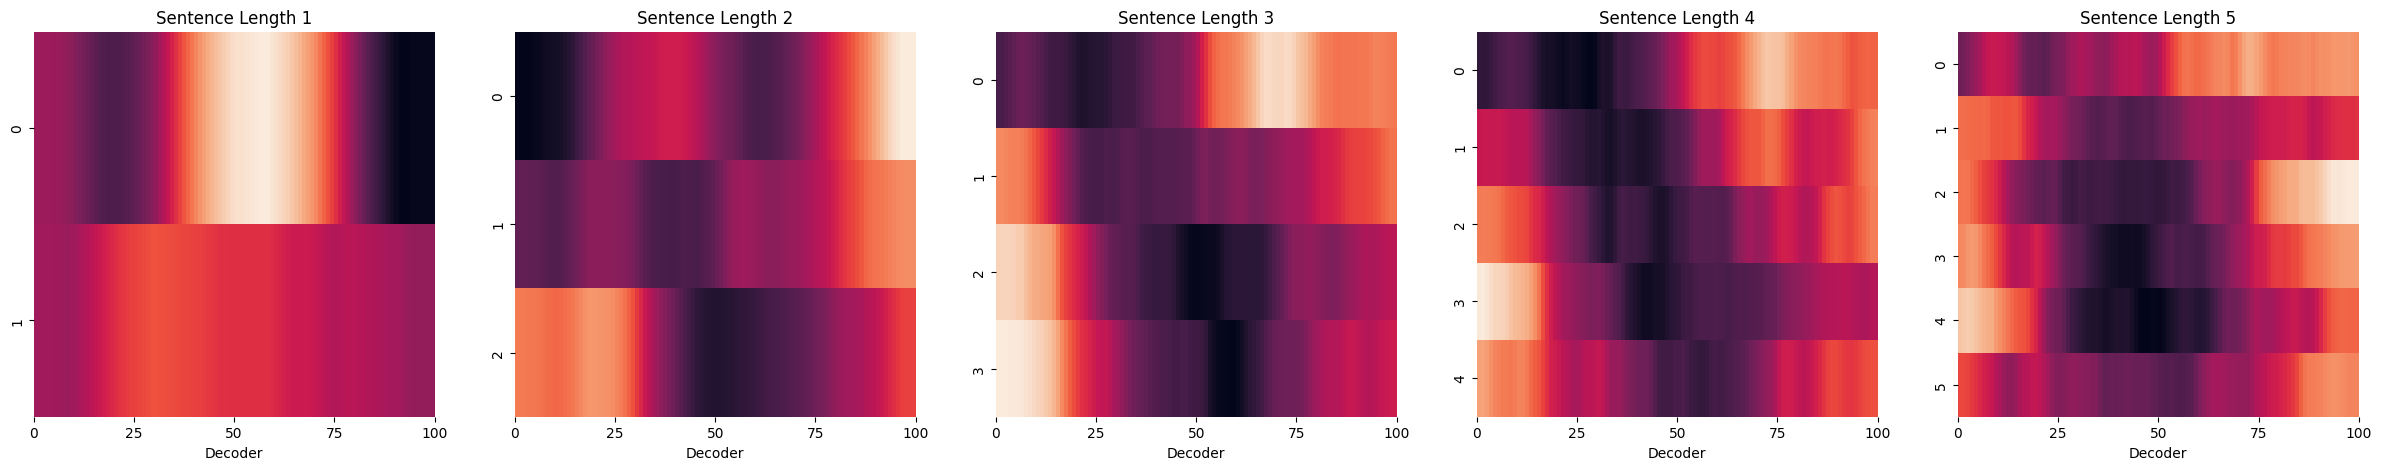
\includegraphics[width=\linewidth]{assets/appendix/avg_decoder_ca_text.png}
        \caption{Average decoder cross-attention scores for sentences with 1 to 5 tokens.}
    \end{subfigure}\hfill
    \begin{subfigure}[b]{\textwidth}
        \centering
        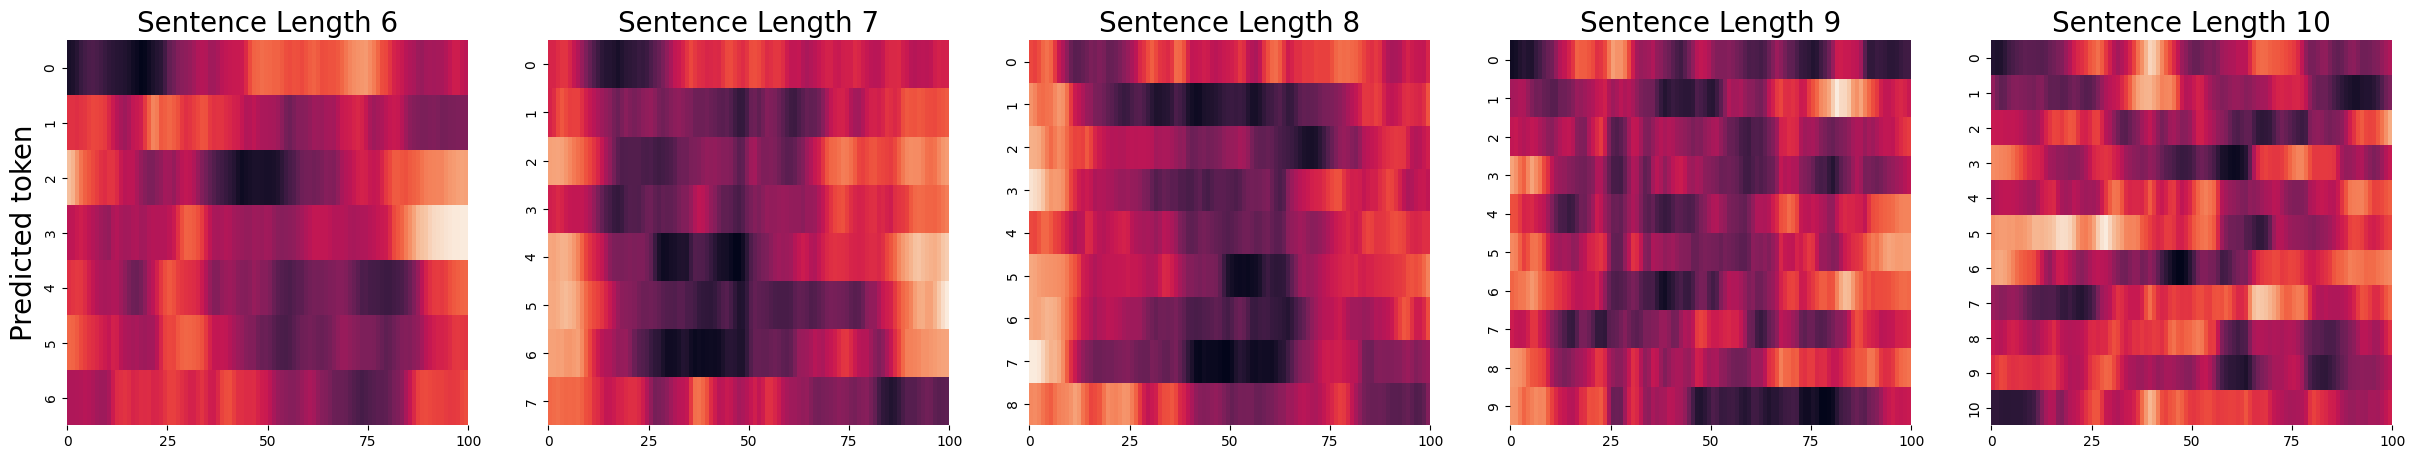
\includegraphics[width=\linewidth]{assets/appendix/avg_decoder_ca_text_2.png}
        \caption{Average decoder cross-attention scores for sentences with 6 to 10 tokens.}
    \end{subfigure}\hfill
    \begin{subfigure}[b]{\textwidth}
        \centering
        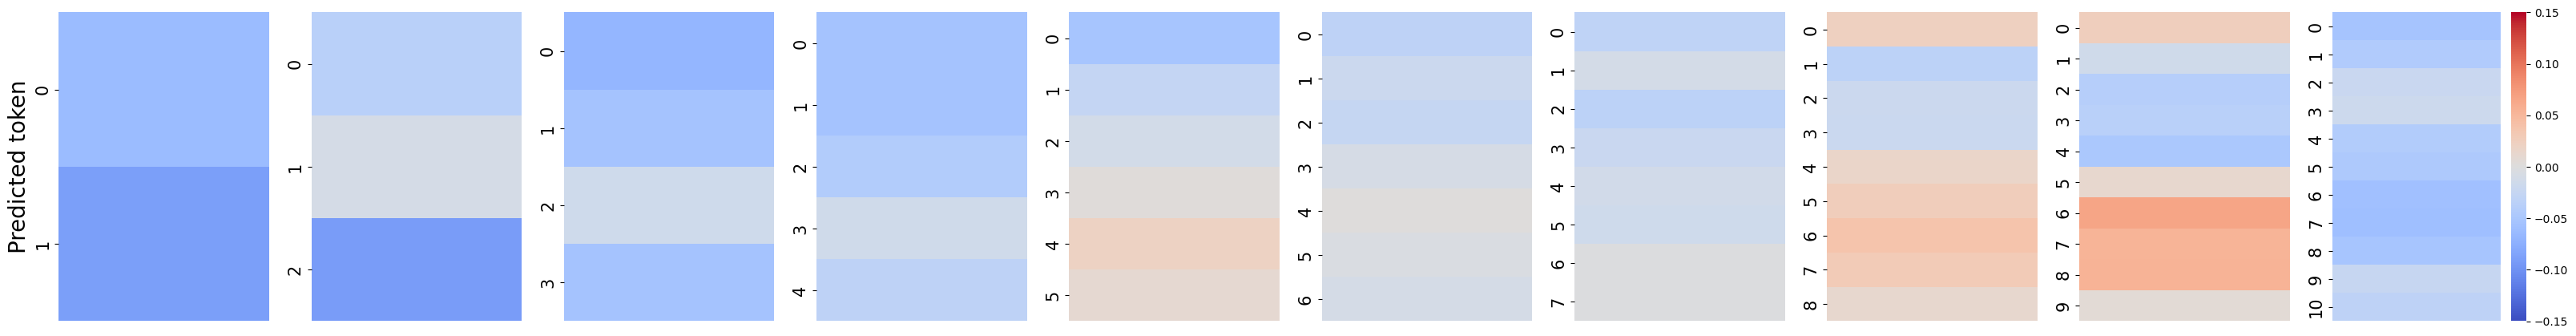
\includegraphics[width=\linewidth]{assets/appendix/sa_ca_diff_text.png}
        \caption{Average differences between self-attention and cross-attention for different sentence lengths.}
    \end{subfigure}
    \begin{subfigure}[b]{\textwidth}
        \centering
        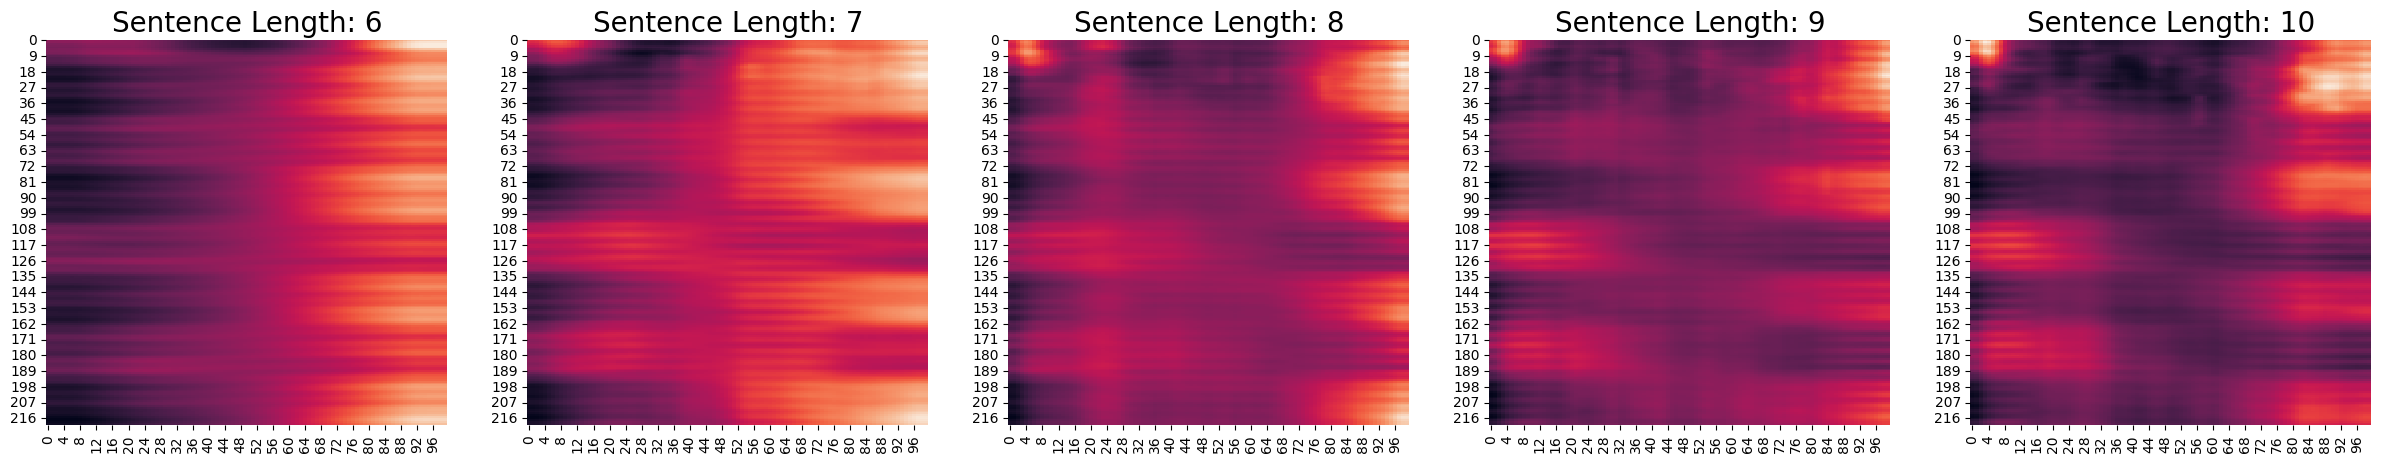
\includegraphics[width=\linewidth]{assets/appendix/avg_encoder_sa_text.png}
        \caption{Average encoder self-attention scores for different sentence lengths.}
    \end{subfigure}\hfill
    \caption{Visualization of dataset-wide results for sign-to-text translation model.}
    \label{fig:text_vis}
\end{figure}